\documentclass{article} % For LaTeX2e
\PassOptionsToPackage{table}{xcolor}
\usepackage{iclr2027_conference,times}

% Optional math commands from https://github.com/goodfeli/dlbook_notation.
\input{math_commands.tex}

\usepackage{hyperref}
\usepackage{url}
\usepackage{algorithm}
\usepackage{algorithmic}
\usepackage{graphicx}
\usepackage{amsmath}
\usepackage{amssymb}
\usepackage{bm}
\usepackage{bbm}
\usepackage{booktabs}
\usepackage{enumitem}
\usepackage{multirow}
\usepackage{array}
\usepackage{xcolor}
\usepackage{caption}
\setlength{\textfloatsep}{10pt plus 2pt minus 2pt}
\setlength{\intextsep}{10pt plus 2pt minus 2pt}
\setlength{\floatsep}{10pt plus 2pt minus 2pt}
\setlength{\abovecaptionskip}{4pt}
\setlength{\belowcaptionskip}{0pt}

\newcommand{\PreserveBackslash}[1]{\let\temp=\\#1\let\\=\temp}
\newcolumntype{C}[1]{>{\PreserveBackslash\centering}p{#1}}

\title{AudioMouth: Articulation-Grounded Structured Generation\\ for Speech-Driven Mouth Animation}

\author{Anonymous Authors}

%\iclrfinalcopy % Uncomment for camera-ready version, but NOT for submission.
\begin{document}

\maketitle

\begin{abstract}
Speech-driven mouth animation aims to produce facial motion synchronized with speech, and existing methods learn this mapping from acoustic features while leaving the articulatory structure of speech implicit in the waveform. Such implicit learning forces the generator to infer which mouth shape a sound requires from acoustics alone, and token-level objectives leave the dynamics and geometry of a complete motion sequence unsupervised. In this paper, we aim to advance speech-driven mouth animation from implicit acoustic regression to explicit articulation-grounded generation. To this end, we propose AudioMouth, which formulates mouth animation as schema-constrained sequence generation with a multimodal language model. AudioMouth first segments long recordings into semantically coherent units sharing temporal boundaries across audio, transcript, phonemes, and target motion, so every phoneme is paired with the motion it produces. Conditioned on these units, AudioMouth generates fixed-schema ARKit coefficient sequences under explicit phoneme-to-articulation grounding, and reweights coefficient-value tokens so frequent near-zero targets no longer dominate supervision. To supervise the trajectory as a whole, AudioMouth further refines the generator with Group Relative Policy Optimization, whose reward measures coefficient accuracy, temporal dynamics, and a simplified lip-geometry discrepancy that reads 3D mouth deformation out of a fixed blendshape basis without rendering or landmark detection. On a subject-disjoint split of BEAT, AudioMouth improves every reported metric over four Audio2ARKit baselines, reducing Fr\'echet distance by 57\% and coefficient MSE by 70\% relative to the strongest of them, and our analyses attribute distributional fidelity to grounding, motion amplitude to balanced supervision, and across-script consistency to geometric feedback.
\end{abstract}

\section{Introduction}
\label{sec:intro}

Speech-driven facial animation aims to generate mouth motion temporally synchronized with speech, supporting digital avatars, game production, and embodied interaction. Recent work has steadily improved the visual quality of talking faces across portrait animation~\citep{ji2021audio,zhang2023sadtalker,xu2024vasa,jiang2024loopy,xu2024hallo}, 3D facial animation~\citep{fan2022faceformer,xing2023codetalker}, and audio-conditioned neural rendering~\citep{guo2021ad,chen2025echomimic,ma2026esgaussianface}. Compact facial representations such as 3D morphable models, FLAME, and blendshape parameterizations provide practical control spaces~\citep{blanz2023morphable,li2017learning,menzel2022automated}, among which ARKit defines semantically meaningful facial action coefficients~\citep{apple_arkit} and has become a standard interface between speech and mouth motion in production. However, how a model decides which mouth shape a given speech sound requires is still left to be discovered from acoustics.

The difficulty lies in the size of the mapping that must be learned from the waveform alone. For instance, a 10-second utterance at 30\,Hz spans 300 frames over 32 mouth-related ARKit channels, so a model must emit 9{,}600 coefficients whose correct values are governed by only about one hundred phonemes. Existing audio-driven methods regress these coefficients from learned acoustic representations~\citep{cudeiro2019voca,richard2021meshtalk,fan2022faceformer,park2023said}, which asks the model to rediscover phoneme identity, phoneme boundaries, and the articulatory action of each phoneme as a by-product of fitting motion. Such implicit learning weakens local correspondence in long utterances, and leaves the model without any notion that a bilabial closure and a wide jaw opening are different articulatory events instead of two nearby points in coefficient space.

Existing attempts to inject linguistic structure into this mapping fall into two lines. Early efforts build viseme inventories and phoneme-to-shape rules~\citep{cohen1993modeling,edwards2016jali,taylor2017deep,zhou2018visemenet}, which make articulation explicit but compress speech into a small discrete inventory, losing the coarticulation that determines how strongly each action is realized. More recently, a line of work injects textual or linguistic cues as auxiliary features of an audio-driven regressor~\citep{fan2022joint,xu2024kmtalk}, and language-aware facial models~\citep{kang2026semanticface,wu2025keyframeface} show that language-aligned supervision helps estimate facial actions. Although these methods enrich the input, the cue is consumed as one more feature vector and the model is never told what action a phoneme category names. In essence, both lines leave the connection between a phonetic unit and a named facial control outside the learning objective. Fortunately, recent multimodal language models~\citep{xu2025qwen3omni} consume audio and text jointly and follow natural-language instructions, which makes it possible to state that connection instead of learning it.

In this paper, we aim to advance speech-driven mouth animation from implicit acoustic regression to explicit articulation-grounded generation, where the model receives the linguistic content, the phonetic units, and the articulatory meaning of those units as inputs, and produces facial controls carrying the same names. Two obstacles stand in the way, namely \emph{boundary mismatch} and \emph{value imbalance}. On the one hand, grounding is only meaningful when a phoneme and the motion it produces occupy the same time span, which long unsegmented recordings do not provide. On the other hand, coefficient values concentrate near zero because most mouth channels stay inactive at any instant, so a token-level objective spends most of its capacity predicting inactivity and under-supervises the large values that shape visible motion. To this end, we propose AudioMouth, which formulates mouth animation as schema-constrained sequence generation with a multimodal language model. Specifically, to resolve boundary mismatch, AudioMouth constructs semantically aligned audio-linguistic units in which one interval selects the audio, transcript, phonemes, and target motion at once, as illustrated in Figure~\ref{fig:overview}. To resolve value imbalance, it applies \emph{distribution-balanced supervision} that downweights frequent near-zero targets so active channels receive proportionally stronger signal, and it generates the coefficient sequence under explicit \emph{articulation grounding} that names the control each phoneme group drives. Since next-token likelihood measures neither how a trajectory moves nor what shape it produces, AudioMouth finally refines the generator with Group Relative Policy Optimization, using a reward over coefficient accuracy, temporal dynamics, and a \emph{simplified lip-geometry discrepancy} (SLMD) that reads 3D mouth deformation out of a fixed blendshape basis without rendering or landmark detection.

Experiments on a subject-disjoint split of BEAT~\citep{liu2022beat} show that AudioMouth improves every reported metric over four Audio2ARKit baselines, reducing Fr\'echet distance by 57\% and coefficient MSE by 70\% relative to the strongest baseline. In summary, our key contributions are three-fold.
\begin{itemize}[leftmargin=1em, itemsep=-1ex, topsep=0ex]
    \item \textbf{Articulation-Grounded Generator:} To the best of our knowledge, AudioMouth is the first framework that generates ARKit mouth trajectories inside a multimodal language model, where phonemes and their articulatory meaning are explicit inputs and the named facial controls are the output schema.
    \item \textbf{Motion-Aware Refinement:} We propose a sequence-level refinement stage whose reward evaluates coefficient accuracy, temporal dynamics, and mouth geometry, and we introduce SLMD to obtain 3D geometric feedback directly from coefficient differences at negligible cost.
    \item \textbf{Strong Performance:} AudioMouth outperforms four Audio2ARKit baselines on all five metrics under a subject-disjoint split, and our analyses attribute the gain to articulation grounding for distributional fidelity, balanced supervision for motion amplitude, and geometric feedback for across-script consistency.
\end{itemize}

\section{Related Work}
\label{sec:related}

\noindent\textbf{Speech-Driven 3D Facial Animation.}\quad
Speech-driven 3D facial animation generates temporally synchronized facial motion from audio, and existing methods are built as direct regression from acoustic features to facial geometry. Early efforts predict vertex displacements, where VOCA~\citep{cudeiro2019voca} produces speaker-specific vertices and MeshTalk~\citep{richard2021meshtalk} learns a categorical latent space covering non-verbal motion, and Transformer-based models later improved long-range temporal modeling~\citep{fan2022faceformer,fan2024unitalker}. Because the audio-to-motion mapping is one-to-many, these regressors average over plausible motions and produce over-smoothed results, which CodeTalker~\citep{xing2023codetalker} mitigates with discrete motion priors and which diffusion-based methods~\citep{park2023said,stan2023facediffuser,sun2025vividtalk} address by modeling motion stochastically. In production settings, Audio2Face-3D~\citep{chung2025audio2face} and related avatar pipelines~\citep{wei2024aniportrait,lin2025cyberhost,sun2024uniavatar,zhen2025teller} provide real-time animation, SentiAvatar~\citep{jin2026sentiavatar} plans at the sentence level, and Ex-Omni~\citep{zhang2026ex} uses an omni-modal model for semantic understanding while delegating coefficient prediction to a lightweight generator. Across this line, the linguistic structure of speech never enters the module that decides mouth shape.

\noindent\textbf{Linguistic and Articulatory Priors.}\quad
Speech articulation is tied to phonetic structure, where bilabial consonants require lip closure, open vowels require larger jaw opening, and phoneme transitions shape the temporal profile of motion~\citep{cohen1993modeling,taylor2012dynamic,edwards2016jali}. Viseme-based methods encode these relations as explicit rules or discrete inventories~\citep{zhou2018visemenet,taylor2017deep,bao2023learning}, which makes articulation interpretable at the cost of collapsing continuous coarticulation into a few categories. Later methods relax this constraint by supplying higher-level cues as auxiliary conditions, including emotion signals~\citep{peng2023emotalk,danvevcek2023emotional,gan2023efficient,jin2026sentiavatar} and linguistic features~\citep{fan2022joint,xu2024kmtalk,wu2025keyframeface}. In these designs the cue enters as a feature vector, so the model still has to learn from scratch what facial action each phonetic category names.

\noindent\textbf{Positioning of AudioMouth.}\quad
The output representation decides whether such grounding is even expressible. Vertex-based representations~\citep{cudeiro2019voca,fan2022faceformer,aloni2025express4d} preserve fine detail but carry no semantics, and parametric models such as FLAME~\citep{li2017learning} gain compactness through PCA axes that are statistical instead of articulatory, so in both cases a prediction cannot be named. ARKit blendshapes~\citep{apple_arkit} instead define named facial actions, which lets one vocabulary describe the articulatory cause and the generated control. In this work, we focus on the articulatory structure of speech, with the goal of making it an explicit part of both the input and the output of mouth-motion generation. Unlike previous approaches that treat linguistic information as auxiliary features of an acoustic regressor, AudioMouth adopts a more deliberate design by generating named ARKit controls inside a multimodal language model that is told which articulatory action each phoneme group requires, and by evaluating the decoded trajectory as a whole through a reward whose geometric term reads out how the predicted coefficients deform the mouth surface.

\section{AudioMouth}
\label{sec:method}

We introduce AudioMouth, which generates mouth-related ARKit trajectories by making the articulatory structure of speech explicit on both sides of the mapping. We first organize long recordings into units where a phoneme and the motion it produces share one time span, then generate a fixed-schema coefficient sequence under phoneme-to-articulation grounding with supervision balanced across coefficient values, and finally refine the generator with a reward computed on the decoded motion. The formulation, the three stages, and inference are introduced as follows.

\begin{figure*}[t]
    \centering
    \vspace{-2mm}
    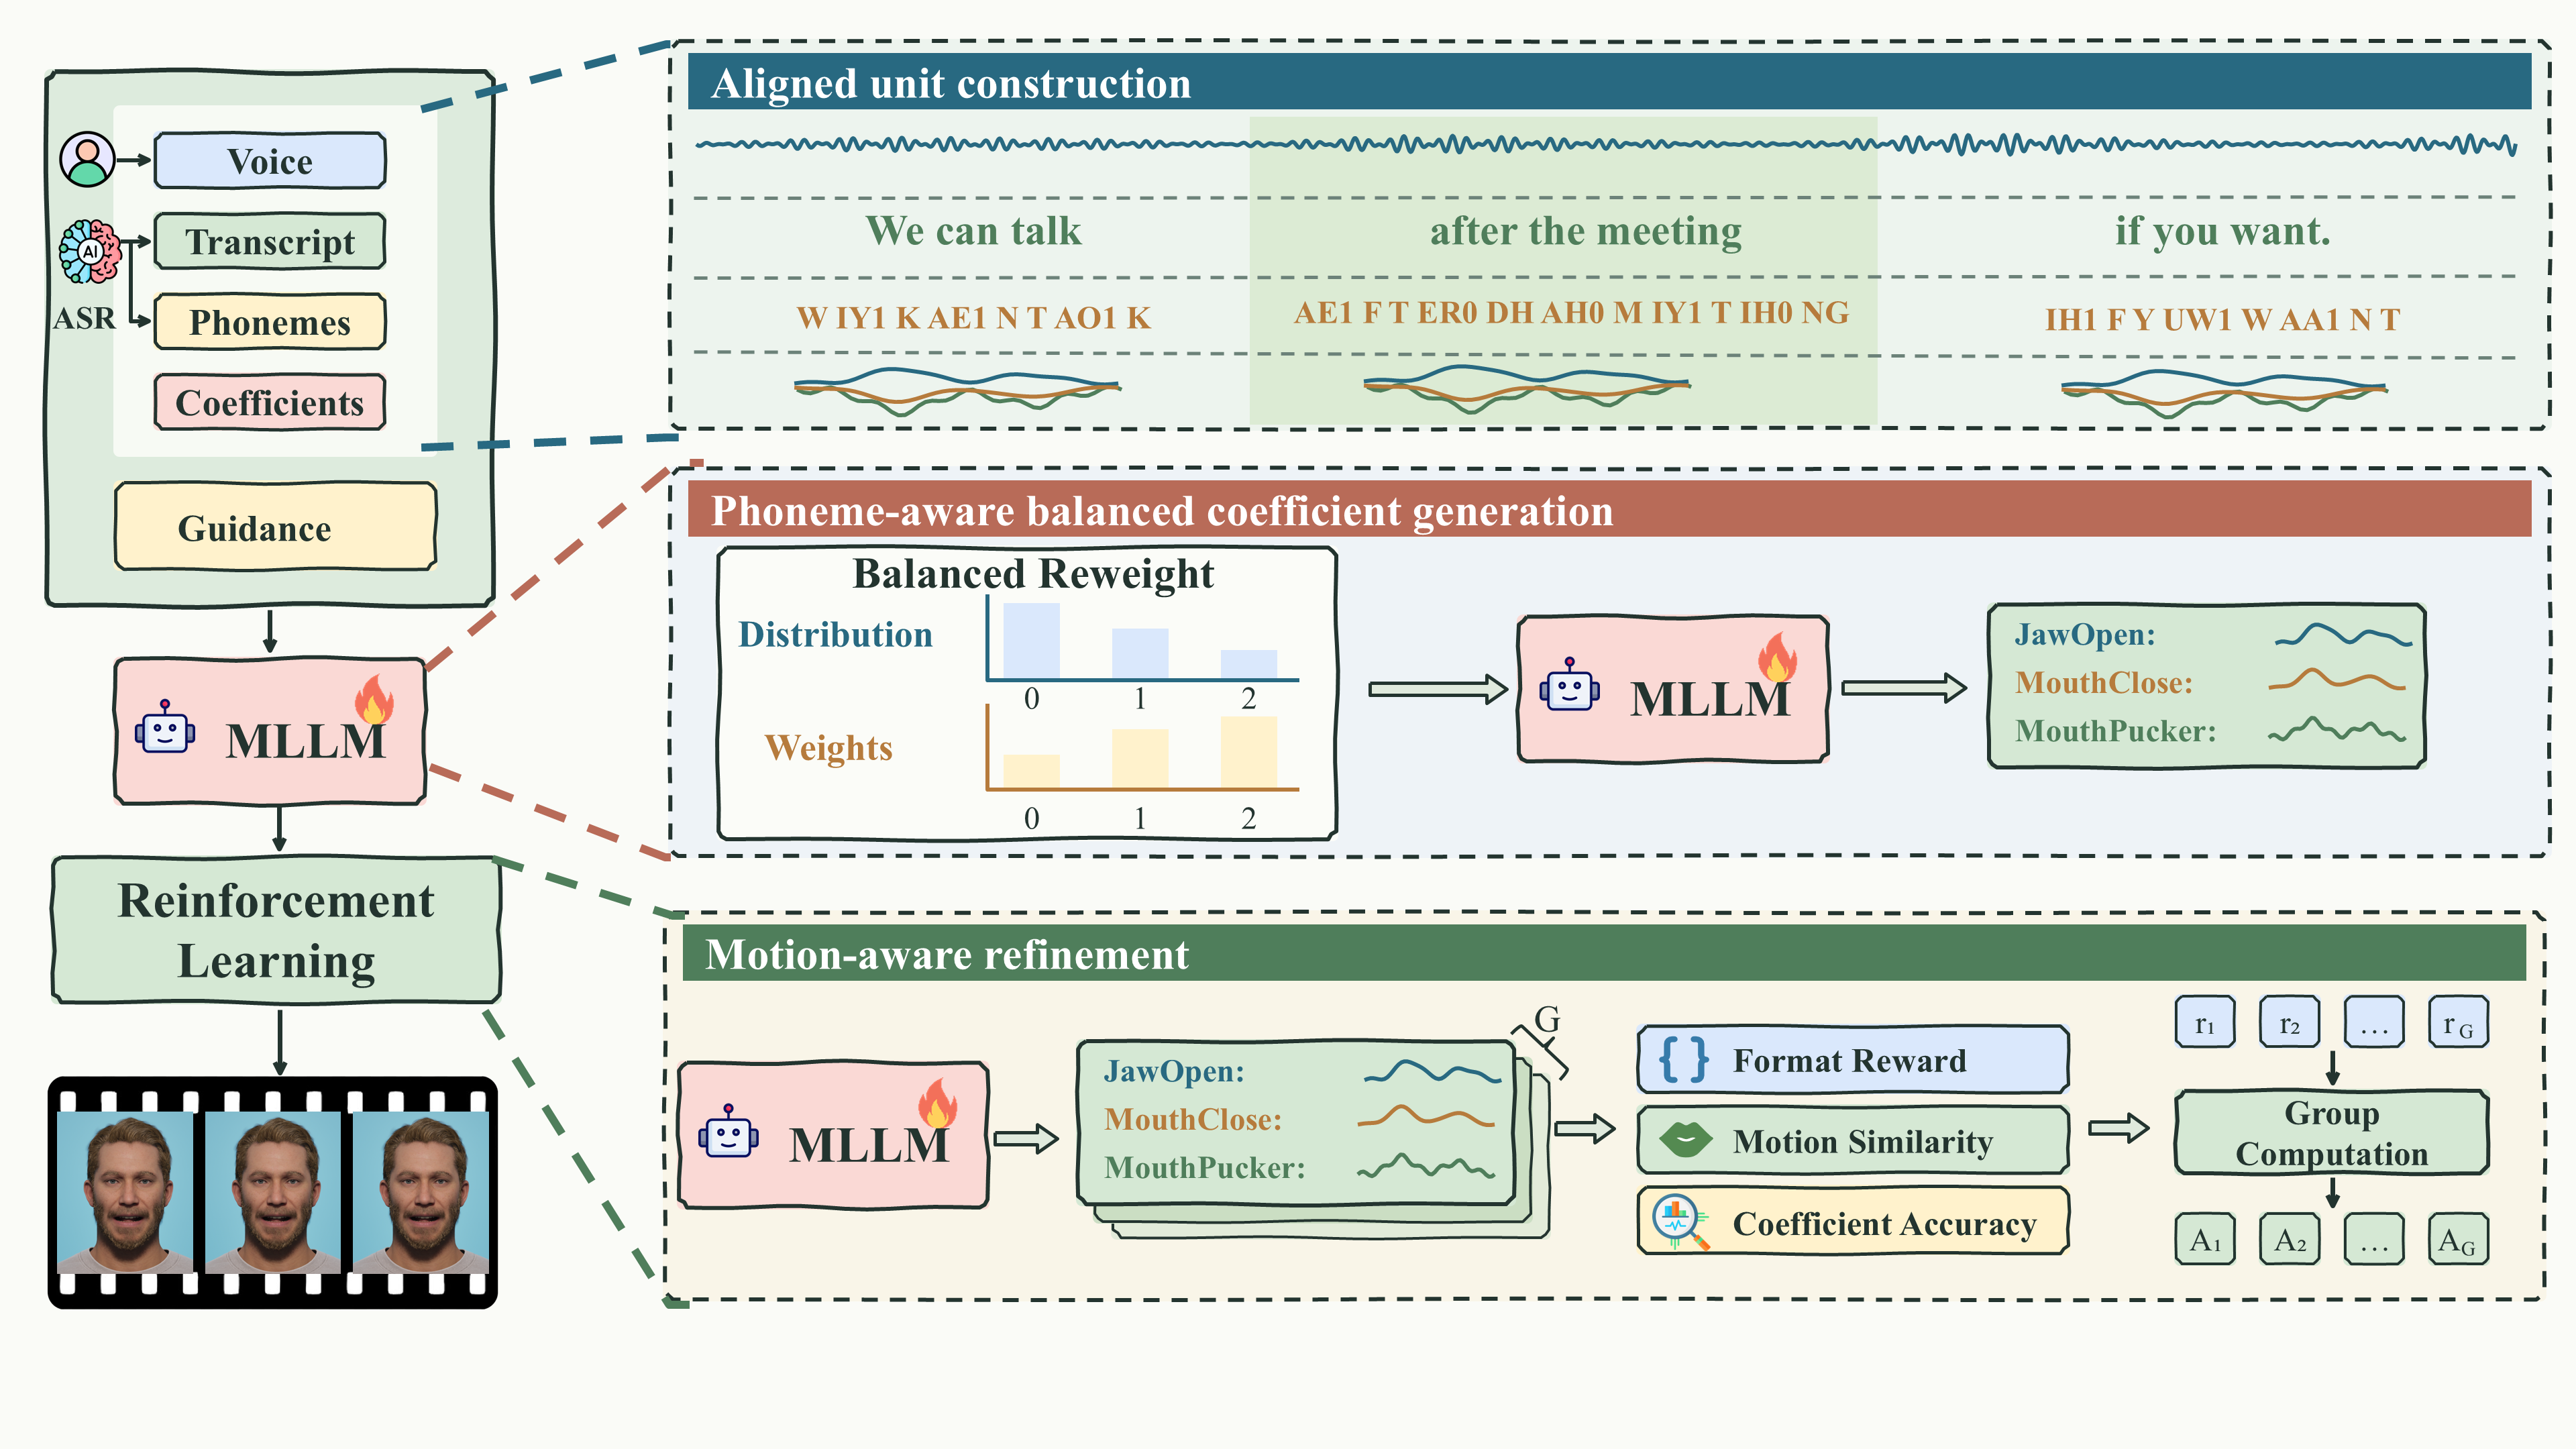
\includegraphics[width=0.80\textwidth]{img/method.png}
    \vspace{-2mm}
    \caption{AudioMouth makes articulation explicit at every stage. Aligned units tie each phoneme to the motion it produces (upper right), grounding and balanced supervision turn those phonemes into named facial controls (middle right), and a motion-level reward including 3D lip geometry corrects what token likelihood cannot measure (lower right).}
    \label{fig:overview}
    \vspace{-3mm}
\end{figure*}

\subsection{Structured Motion Generation}
\label{sec:formulation}

Given a speech waveform $\mathcal{A}\!=\!\{a_{n}\}_{n=1}^{N}$ of $N$ samples, our goal is to predict a synchronized coefficient sequence $\mathcal{V}\!=\!\{v_{t}\}_{t=1}^{T}$ over $T$ motion frames, where each $v_{t}\!\in\!\mathbb{R}^{K}$ holds the $K\!=\!32$ mouth-related ARKit controls~\citep{apple_arkit} retained by SAiD~\citep{park2023said}. We divide each recording into $J$ aligned units, so unit $j$ carries the inputs and target
\begin{gather}
    \mathcal{X}^{j}=\left(\mathcal{A}^{j},\,\mathcal{W}^{j},\,\mathcal{P}^{j},\,\mathcal{G}\right),\quad
    \mathcal{Y}^{j}=f_{\mathrm{json}}\!\left(\mathcal{V}^{j}\right), \label{eq:unit}
\end{gather}
where $\mathcal{W}^{j}$ and $\mathcal{P}^{j}$ are the transcript and phoneme sequence of the audio segment $\mathcal{A}^{j}$, $\mathcal{G}$ is the phoneme-to-articulation grounding of Sec.\ref{sec:stage2}, $\mathcal{V}^{j}$ is the target motion, and $f_{\mathrm{json}}(\cdot)$ serializes each ARKit channel into a predefined key holding that channel in temporal order. A fixed schema turns animation into generation without a regression head. The generator $f_{\mathrm{gen}}(\cdot)$ with parameters $\theta$ models $\mathcal{Y}^{j}\!=\!(y_{1},\cdots,y_{M_{j}})$ autoregressively as
\begin{gather}
    p_{\theta}\!\left(\mathcal{Y}^{j}\mid\mathcal{X}^{j}\right)=\prod_{m=1}^{M_{j}}p_{\theta}\!\left(y_{m}\mid y_{<m},\mathcal{X}^{j}\right), \label{eq:ar}
\end{gather}
where $M_{j}$ is the output length and $y_{<m}$ the preceding tokens. Two requirements follow, since conditioning only helps when it covers the same time span as the target, and the likelihood in Eq.(\ref{eq:ar}) is blind to the value distribution of the targets and to the shape of the decoded trajectory.

\subsection{Semantic-Aligned Audio-Linguistic Units}
\label{sec:stage1}

\noindent\textbf{Boundary-Shared Unit Construction.}\quad
To make a phoneme informative about motion, the phoneme and the motion must refer to the same interval, which a long recording does not supply. We therefore build units whose boundaries are shared by all four signals, using automatic speech recognition $f_{\mathrm{asr}}(\cdot)$~\citep{gao2023funasr,zhang2022paddlespeech} for the transcript and word-level timestamps $\tau$, and semantic segmentation $f_{\mathrm{seg}}(\cdot)$~\citep{frohmann2024segment} for coherent utterances,
\begin{gather}
    \left(\tilde{\mathcal{W}},\tau\right)=f_{\mathrm{asr}}\!\left(\mathcal{A}\right),\quad
    \left\{\mathcal{W}^{j}\right\}_{j=1}^{J}=f_{\mathrm{seg}}\!\left(\tilde{\mathcal{W}}\right). \label{eq:seg}
\end{gather}
The first and last words of $\mathcal{W}^{j}$ determine one interval through $\tau$, which selects $\mathcal{A}^{j}$, $\mathcal{P}^{j}$, and, during training, $\mathcal{V}^{j}$. Cutting at semantic boundaries instead of fixed-length windows keeps every unit a complete utterance, because a window that splits a word hands the generator a phoneme whose articulatory consequence lies outside the unit. At inference the same construction runs without the motion branch.

\subsection{Articulation-Grounded Balanced Generation}
\label{sec:stage2}

\noindent\textbf{Articulation Grounding.}\quad
Aligned phonemes tell the model when a speech sound occurs but not what the mouth does to produce it, and an audio-driven regressor has to recover that relation from motion data alone. AudioMouth instead states it. Specifically, the grounding $\mathcal{G}$ in Eq.(\ref{eq:unit}) is a fixed statement mapping phonetic categories to the named ARKit controls they drive, connecting bilabial consonants to lip closure and open vowels to larger jaw opening. Since the output schema reuses those control names, the model carries the relation from instruction to generated key instead of inferring it, while the audio stays responsible for how strongly each action is realized. We call this division \emph{articulation grounding}, and it is why phonemes and their meaning are supplied together.

\noindent\textbf{Distribution-Balanced Supervision.}\quad
Grounded conditioning still leaves the objective unbalanced, because most mouth channels are inactive at any instant and their near-zero values dominate the token stream. Under the plain likelihood of Eq.(\ref{eq:ar}) the model is rewarded most for predicting inactivity, so the large values that produce visible motion contribute a small fraction of the gradient. We therefore reweight the loss with a fixed function $\omega(\cdot)$ that downweights the frequent low-valued tokens, giving
\begin{gather}
    \mathcal{L}_{\mathrm{db}}=-\sum_{m=1}^{M_{j}}\omega\!\left(y_{m}\right)\log p_{\theta}\!\left(y_{m}\mid y_{<m},\mathcal{X}^{j}\right), \label{eq:db}
\end{gather}
where $\omega(y_{m})$ depends only on the value a coefficient token carries and equals one on every schema token, so keys and punctuation keep their weight and the output format is unaffected. The weighting is one monotone table, fixed before training and shared across all channels and all experiments, with values in Appendix~\ref{app:json}. Supervised fine-tuning with Eq.(\ref{eq:db}) yields $\theta_{\mathrm{sft}}$, which initializes refinement.

\subsection{Motion-Aware Refinement with Geometric Feedback}
\label{sec:stage3}

Even a well-balanced token objective scores a trajectory one value at a time, so it cannot separate a sequence that moves like the reference from one reaching similar values through implausible motion, and cannot tell which coefficient errors change the visible mouth. We close this gap by refining $\theta_{\mathrm{sft}}$ with Group Relative Policy Optimization (GRPO)~\citep{shao2024deepseekmath} against a reward computed on the decoded motion, where we sample $G$ candidates per input $\mathcal{X}^{j}$, parse each into a trajectory through $f_{\mathrm{parse}}(\cdot)$, and compare it with the reference $\mathcal{V}^{j}$.

\noindent\textbf{Simplified Lip-Geometry Discrepancy.}\quad
Coefficient-wise errors treat the $K$ controls as independent while the visible mouth is their joint result, so two candidates with equal coefficient error can differ greatly in shape, and rendering each candidate to measure that difference is far too slow inside a sampling loop. We therefore introduce the \emph{simplified lip-geometry discrepancy} (SLMD), which reads the shape difference out of the coefficients through a fixed blendshape basis. Let $\mathbf{C}^{p},\mathbf{C}^{g}\!\in\!\mathbb{R}^{T\times K}$ denote the candidate and reference sequences, and let $\mathbf{b}_{k,m}\!\in\!\mathbb{R}^{3}$ be the displacement the $k$-th blendshape applies to mouth-region vertex $m\!\in\!\mathcal{M}$ relative to the neutral mesh. Since both sequences are driven from the same neutral geometry, the neutral term cancels and the per-vertex displacement difference $\delta\mathbf{x}_{t,m}=f_{\mathrm{geo}}(\mathbf{C}^{p}\!-\!\mathbf{C}^{g})$ and the resulting discrepancy are
\begin{align}
    \delta\mathbf{x}_{t,m}&=\sum_{k=1}^{K}\left(c^{p}_{t,k}-c^{g}_{t,k}\right)\mathbf{b}_{k,m}, \label{eq:slmd_disp}\\
    \mathcal{L}_{\mathrm{slmd}}&=\frac{\sum_{t=1}^{T}\sum_{m\in\mathcal{M}}w_{m}\left\|\delta\mathbf{x}_{t,m}\right\|_{2}}{T\sum_{m\in\mathcal{M}}w_{m}}, \label{eq:slmd}
\end{align}
where the fixed vertex weights $w_{m}$ emphasize the lip region while retaining lower-weighted surrounding vertices, and $T$ is the compared length. SLMD therefore costs one matrix product per candidate, couples all $K$ controls through their shared effect on the surface, and stays in the coefficient domain, which keeps it independent of the rendered-video landmark metric used for evaluation.

\noindent\textbf{Motion-Level Reward.}\quad
Mouth quality involves both the shape at each instant and how that shape evolves, so SLMD alone is not sufficient. We combine it with the coefficient error $\mathcal{L}_{\mathrm{mse}}$ and the first- and second-order temporal difference discrepancies $\mathcal{L}_{\mathrm{vel}}$ and $\mathcal{L}_{\mathrm{acc}}$, which compare how the candidate changes against how the reference changes instead of penalizing movement itself. The four terms live on different numerical scales, so each is mapped to a bounded score before aggregation, giving
\begin{align}
    S_{q}=\left(1+\mathcal{L}_{q}/s_{q}\right)^{-1},\quad
    r_{\mathrm{motion}}=\sum_{q\in\mathcal{Q}}\lambda_{q}S_{q},\quad \mathcal{Q}=\left\{\mathrm{mse},\mathrm{vel},\mathrm{acc},\mathrm{slmd}\right\}, \label{eq:reward}
\end{align}
where each scale $s_{q}$ is the median of $\mathcal{L}_{q}$ measured once on reference data so the four scores occupy a comparable range, and the nonnegative weights $\lambda_{q}$ sum to one. Invalid schema instances receive a fixed negative reward and valid candidates of the wrong length are penalized in proportion to their length error, which keeps format compliance and duration control inside one signal. All scales, weights, and penalties are fixed once and reused across every experiment, with values in Appendix~\ref{app:refinement}.

\noindent\textbf{Group-Relative Policy Update.}\quad
To turn these absolute rewards into a learning signal without a value network, we normalize them within each sampled group as $\hat{A}_{i}=(r_{i}-\bar{r})/(\sigma_{r}+\epsilon)$, where $\bar{r}$ and $\sigma_{r}$ are the group mean and standard deviation and $\epsilon$ ensures numerical stability. Since all $G$ candidates answer the same input, the comparison isolates what the policy did differently on this utterance and favors the candidate whose motion is closer to the reference in shape and dynamics, so $\theta_{\mathrm{grpo}}$ keeps the schema learned during supervised fine-tuning and adds the sequence-level preference that token likelihood cannot express.

\noindent\textbf{Inference.}\quad
Given test speech, we build input units as in Sec.\ref{sec:stage1} and generate one coefficient JSON per unit with $\theta_{\mathrm{grpo}}$. The decoded segments are concatenated in temporal order and passed through $f_{\mathrm{post}}(\cdot)$, which suppresses residual jitter and the small discontinuities appearing where two independently generated units meet, giving
\begin{gather}
    \hat{\mathcal{V}}=f_{\mathrm{post}}\!\left(\mathrm{Concat}\!\left(\left\{f_{\mathrm{parse}}\!\left(\hat{\mathcal{Y}}^{j}\right)\right\}_{j=1}^{J}\right)\right). \label{eq:infer}
\end{gather}
Algorithm~\ref{alg:framework} summarizes the procedure, and Appendix~\ref{app:additional} verifies that $f_{\mathrm{post}}(\cdot)$ complements refinement instead of substituting for it.

\section{Experiments}
\label{sec:exp}

\subsection{Experimental Setting}
\label{sec:setting}

\noindent\textbf{Benchmark.}\quad We conduct experiments on BEAT~\citep{liu2022beat}, which pairs natural speech with ARKit coefficients captured at 60\,Hz and is therefore directly usable for an Audio2ARKit comparison. We use its English subset and screen it by rendering the captured coefficients against the audio, discarding sequences with tracking failures or audible misalignment, since a reference that does not match its own audio cannot support training or evaluation. The retained data are split by speaker into 176 training, 40 validation, and 61 test sequences, and semantic segmentation yields 15{,}655 training, 2{,}858 validation, and 3{,}000 test units. Appendix~\ref{app:dataset} details the procedure.

\noindent\textbf{Metrics.}\quad We report five metrics covering accuracy, distribution, and appearance, where MSE and MAE measure frame-level coefficient error. Fr\'echet distance (FD) measures the discrepancy between predicted and reference motion distributions in a feature space, and Wasserstein inception distance (WInD) follows the protocol of SAiD~\citep{park2023said}. Lip landmark distance (LMD) measures the mean Euclidean distance between 2D mouth landmarks in paired rendered videos, and is the only metric outside the coefficient domain, which makes it independent of the geometric term inside our reward.

\noindent\textbf{Baselines.}\quad We compare AudioMouth with four Audio2ARKit methods, namely LAM-A2E~\citep{lam}, NVIDIA Audio2Face-3D~\citep{chung2025audio2face}, SAiD~\citep{park2023said}, and SentiAvatar~\citep{jin2026sentiavatar}, covering real-time production pipelines, diffusion-based generation, and sentence-level planning. SAiD is fine-tuned from its public checkpoint on our training split, while the other three are evaluated with released weights because their training code or data is unavailable. Two asymmetries follow. The three unadapted baselines never see our speakers, and all four consume audio alone while AudioMouth also consumes the transcript and phonemes its formulation requires. Table~\ref{tab:main} therefore compares formulations as they are distributed, and the Audio Only ablation of Sec.\ref{sec:ana_conditioning} is the matched-input reference under our own backbone and data.

\noindent\textbf{Configuration.}\quad We build AudioMouth on Qwen3-Omni-30B-A3B-Instruct~\citep{xu2025qwen3omni} and adapt it with LoRA~\citep{hu2021lora} on the language decoder, keeping the audio encoder and multimodal alignment modules frozen so adaptation concerns only how motion is generated. Preprocessing combines automatic speech recognition with SAT~\citep{frohmann2024segment}. Supervised fine-tuning and GRPO each run for four epochs, refinement samples six candidates per prompt, all training and inference use NVIDIA A100 GPUs, and predictions are rendered with MetaHuman~\citep{metahuman}. Appendix~\ref{app:training} reports the full configuration.

\subsection{Main Results}
\label{sec:main_results}

\begin{table}[t]
\centering
\caption{AudioMouth improves every metric over four Audio2ARKit methods on the subject-disjoint BEAT test split, with the largest margins on the distributional metrics FD and WInD. All metrics are lower-is-better. FD, WInD, and LMD are mean $\pm$ sample standard deviation across evaluation scripts, \textbf{bold} marks the best result per column, and \textcolor{blue}{$_{-x\%}$} is the relative reduction over the strongest baseline in that column.}
\label{tab:main}
\vspace{-1mm}
\scriptsize
{\renewcommand{\arraystretch}{1.12}
\begin{tabular*}{\textwidth}{@{\extracolsep{\fill}} lccccc @{}}
\toprule
\textbf{Methods} & \textbf{MSE $\downarrow$} & \textbf{MAE $\downarrow$} & \textbf{FD $\downarrow$} & \textbf{WInD $\downarrow$} & \textbf{LMD $\downarrow$} \\
\midrule
LAM-A2E                       & $0.023$ & $0.109$ & $38.403 \pm 10.149$ & $41.751 \pm 10.885$ & $7.648 \pm 0.497$ \\
Audio2Face-3D                 & $0.020$ & $0.106$ & $25.228 \pm 3.560$  & $29.879 \pm 4.454$  & $7.879 \pm 0.438$ \\
SAiD                          & $0.021$ & $0.108$ & $58.357 \pm 21.580$ & $62.256 \pm 21.911$ & $7.651 \pm 0.504$ \\
SentiAvatar                   & $0.022$ & $0.106$ & $40.609 \pm 10.277$ & $42.153 \pm 10.542$ & $8.131 \pm 1.005$ \\
\midrule
\rowcolor{gray!15}
\textbf{AudioMouth} & $\mathbf{0.006}$\,\textcolor{blue}{$_{-70\%}$} & $\mathbf{0.053}$\,\textcolor{blue}{$_{-50\%}$} & $\mathbf{10.820 \pm 2.635}$\,\textcolor{blue}{$_{-57\%}$} & $\mathbf{16.513 \pm 3.584}$\,\textcolor{blue}{$_{-45\%}$} & $\mathbf{6.249 \pm 0.723}$\,\textcolor{blue}{$_{-18\%}$} \\
\bottomrule
\end{tabular*}
}
\vspace{-4mm}
\end{table}

\noindent\textbf{Capability on Speech-Driven Coefficient Prediction.}\quad
We first evaluate AudioMouth on the BEAT test split to assess its \emph{coefficient-level articulation accuracy}, where every method receives the same speech and predicts the same 32 channels over the same speaking intervals. We compare it with the four Audio2ARKit baselines of Sec.\ref{sec:setting}. As shown in Table~\ref{tab:main}, AudioMouth achieves state-of-the-art performance among Audio2ARKit methods on all five metrics, substantially reducing MSE by 70\% and Fr\'echet distance by 57\% relative to the strongest baseline in each column. More importantly, the gains are not uniform across metric types. Frame-level MSE and MAE separate the four baselines by at most 15\%, which indicates that predicting the dominant near-zero coefficients is easy for any reasonable regressor and that frame-level error alone cannot distinguish these methods. The distributional FD and WInD spread the same baselines over a factor of two, showing that what differs between them is whether the predicted motion occupies the same region of motion space as real speech. In contrast, AudioMouth improves most on exactly these distributional metrics, which stems from articulation grounding, since naming the control a phoneme drives constrains which channels move and not only how much error each channel accumulates. Its FD standard deviation is also the smallest of all methods, so the advantage holds across scripts. Overall, AudioMouth's strong results on BEAT highlight its advanced capability in producing mouth motion whose channel activation pattern matches real articulation.

\begin{figure*}[t]
    \centering
    \vspace{-2mm}
    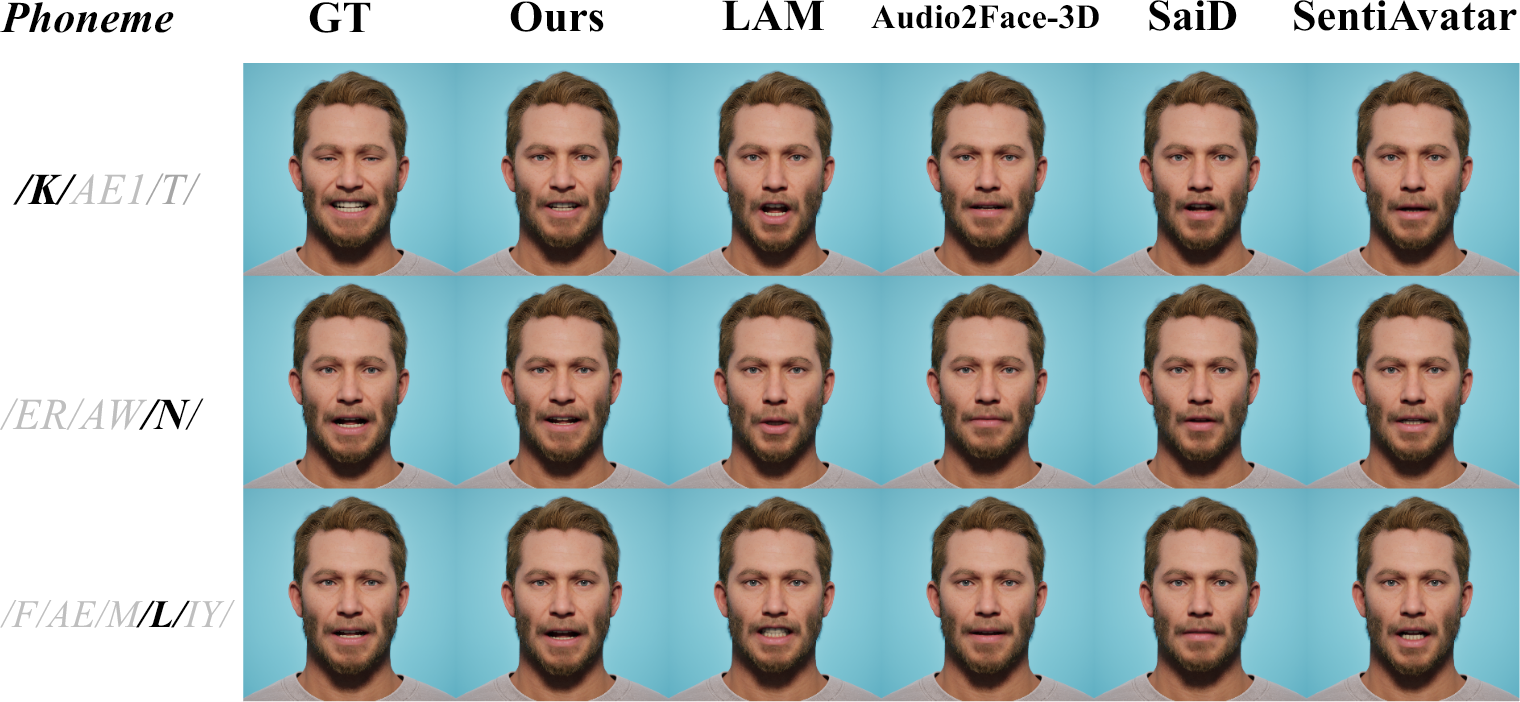
\includegraphics[width=0.9\linewidth]{comparison.png}
    \vspace{-2mm}
    \caption{AudioMouth reproduces the articulatory target of each phoneme, closing the lips on the bilabial in ``family'' and opening the jaw on the open vowel in ``cat'', where baselines keep a partially open, weakly differentiated mouth shape. The leftmost column shows the phoneme context with the active phoneme in bold.}
    \label{fig:comparison}
    \vspace{-3mm}
\end{figure*}

\noindent\textbf{Capability on Rendered Mouth Appearance.}\quad
Coefficient accuracy is only useful if it survives rendering, so we render every prediction with MetaHuman and measure LMD against the rendered reference, the one metric computed outside the coefficient domain. As shown in Table~\ref{tab:main}, AudioMouth reduces LMD by 18\% relative to the best baseline, a smaller margin than the 57\% it achieves on FD. This narrower margin stems from how the two metrics are formed, because LMD averages a landmark distance over all frames and is dominated by the many frames in which the mouth is nearly closed for every method, while FD is sensitive to the shape of the whole motion distribution. Figure~\ref{fig:comparison} shows where the remaining difference is visible. On the bilabial in ``family'' the baselines leave a gap between the lips, and on the open vowel in ``cat'' they produce a moderate opening for a sound requiring a wide one, whereas AudioMouth reaches the articulatory target in both cases. In contrast, AudioMouth is told that bilabials close the lips, so it reproduces a named articulatory event instead of a numerical average over acoustically similar sounds. Overall, AudioMouth's strong results under rendering highlight its advanced capability in carrying coefficient-level accuracy through to the visible face, with the clearest gains on the phonemes whose articulation is most constrained.

\section{Analysis}
\label{sec:analysis}

\begin{figure}[t]
    \centering
    \vspace{-3mm}
    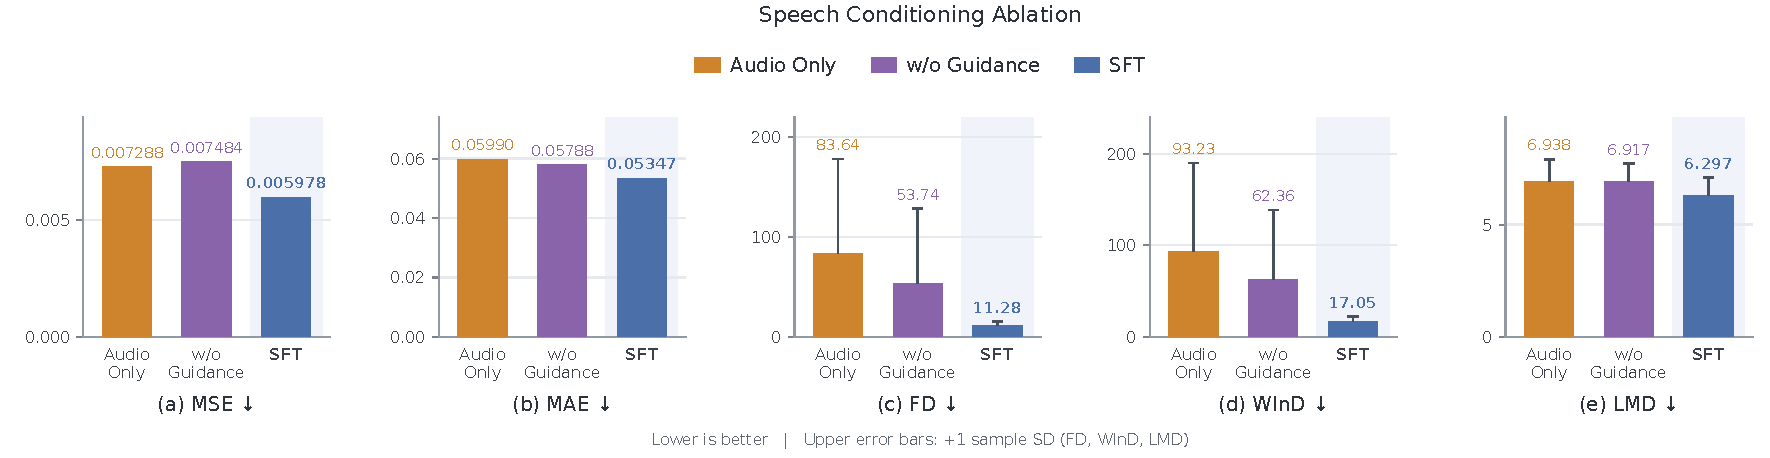
\includegraphics[width=0.82\linewidth]{figures/ablation_conditioning_wide.pdf}\\[0.6mm]
    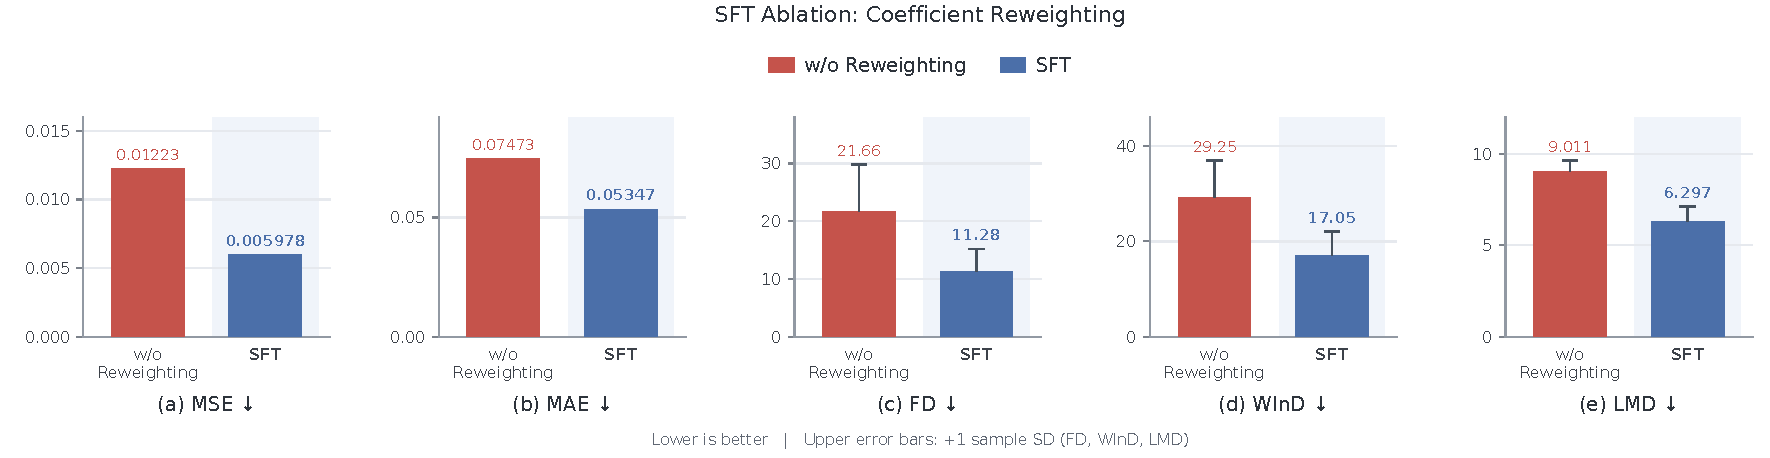
\includegraphics[width=0.82\linewidth]{figures/ablation_reweighting_wide.pdf}
    \vspace{-2mm}
    \caption{The two supervised-stage components act on different failure modes. Removing articulation grounding (top) costs little frame-level error while inflating the distributional metrics and their across-script variance by an order of magnitude, whereas removing the balanced objective (bottom) keeps motion in the right channels yet shrinks its amplitude, which doubles frame-level error and yields the worst rendered landmark distance we measure. Lower is better, and error bars show one sample standard deviation.}
    \label{fig:ablation_sft}
    \vspace{-5mm}
\end{figure}

\subsection{Ablation Study on Articulation Grounding}
\label{sec:ana_conditioning}

To verify that the gain of AudioMouth comes from articulation grounding instead of from the capacity of the multimodal backbone, we ablate the linguistic inputs while holding the backbone, the training data, the objective, and the post-processing identical. The full model receives audio, transcript, phonemes, and the grounding statement. The w/o Guidance variant keeps transcript and phonemes but deletes the statement naming which control each phoneme group drives, and the Audio Only variant deletes all three, which reduces the model to a structured audio-to-coefficient regressor.

As shown in the top row of Figure~\ref{fig:ablation_sft}, the three settings differ by at most a quarter in MSE and about a tenth in MAE, yet by almost an order of magnitude in FD and WInD, where the full model significantly reduces FD by about 79\% relative to w/o Guidance. Notably, the across-script standard deviation grows from a few units for the full model to a value comparable to the mean itself once grounding is removed, a size that cannot describe uniformly degraded motion and instead indicates that the ungrounded variants track speech acceptably on most scripts and then drift badly on some of them. Without a statement connecting phonemes to named controls, the model has no anchor telling it which channels a sound may activate, so when acoustic evidence is ambiguous it settles on a channel combination that is numerically close yet articulatorily wrong. Phonemes alone recover part of that anchor by narrowing the set of sounds produced, which is why w/o Guidance already cuts the FD of Audio Only by more than a third while the two stay comparable at the frame level. The results show that the benefit of linguistic conditioning comes mainly from naming the articulatory action and not from supplying extra input features, demonstrating the advantage of articulation grounding over feature-level linguistic conditioning.

\subsection{Superiority of Distribution-Balanced Supervision}
\label{sec:ana_reweight}

To verify that reweighting coefficient-value tokens addresses the value imbalance identified in Sec.\ref{sec:stage2}, we compare the balanced objective of Eq.(\ref{eq:db}) with a w/o Reweighting variant assigning unit weight to every coefficient-value token, holding conditioning, schema, and post-processing fixed so the comparison isolates the objective.

As shown in the bottom row of Figure~\ref{fig:ablation_sft}, removing the weighting roughly doubles MSE and, more strikingly, raises LMD above every baseline in Table~\ref{tab:main}, including methods whose own coefficient error is nearly twice as large. This combination is only possible for one reason. Under unit weights the loss is dominated by frequent near-zero targets, so the model converges to a solution that is nearly always right about inactivity and too small whenever motion is required. The rendered face therefore moves in the right places and by too little, which a landmark metric on pixels punishes far more than a coefficient metric on numbers. The distributional metrics agree, since FD degrades but stays well below the ungrounded variants of Sec.\ref{sec:ana_conditioning}, so the channel pattern learned from grounding survives while its amplitude does not. The results show that grounding and balanced supervision act on different failure modes, where the former decides which controls move and the latter decides how far, demonstrating the advantage of combining both in a language model that emits quantized motion.

\begin{figure}[t]
    \centering
    \vspace{-3mm}
    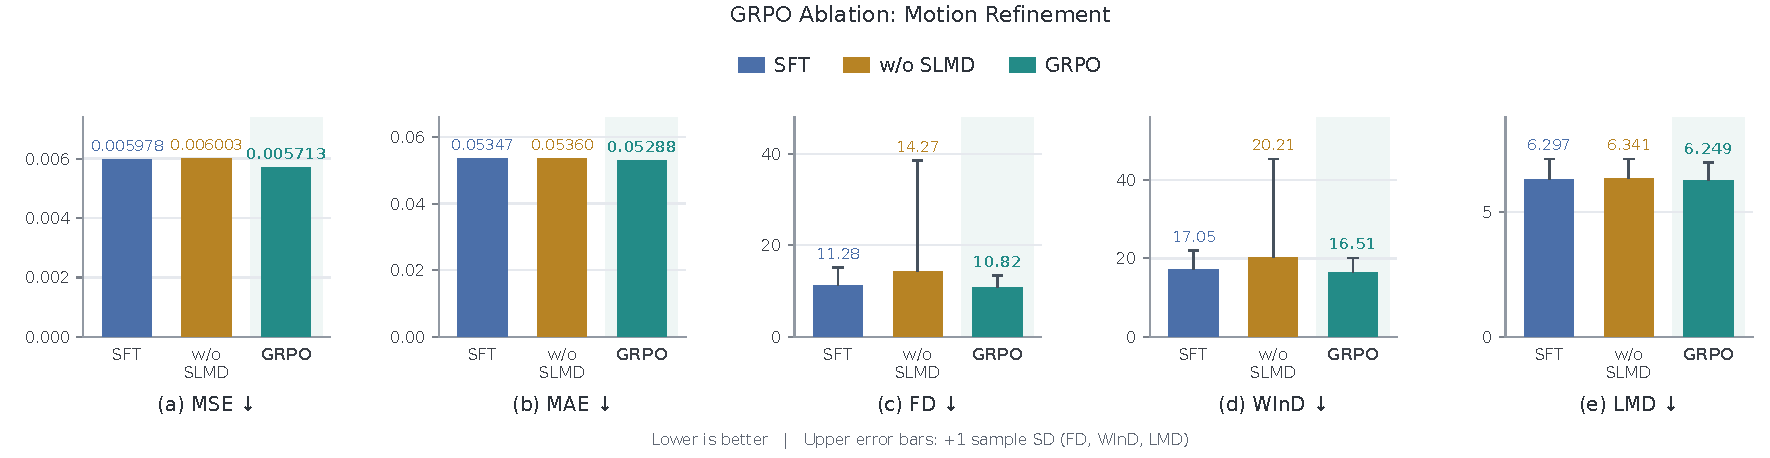
\includegraphics[width=0.82\linewidth]{figures/ablation_motion_wide.pdf}
    \vspace{-2mm}
    \caption{Motion-aware refinement improves consistency more than means. Full refinement gives small gains on every metric and cuts across-script FD deviation by a third, while dropping the geometric term makes refinement unstable.}
    \label{fig:ablation_motion}
    \vspace{-5mm}
\end{figure}

\subsection{Effect of Motion-Aware Refinement and Geometric Feedback}
\label{sec:ana_grpo}

To verify that sequence-level feedback adds something token-level supervision cannot provide, we compare the supervised and refined generators under an identical post-processing setting, so any difference is attributable to the GRPO stage alone. As shown in Figure~\ref{fig:ablation_motion}, refinement improves all five metrics, and the gain in the means is modest at roughly 4\% on MSE and FD. We do not claim more, because differences of this size approach the resolution of a comparison over a few dozen scripts.

In particular, the effect that is not modest is dispersion, since refinement cuts the across-script FD standard deviation by about a third and makes the refined model noticeably more uniform than the supervised model that produced its own initialization. This improvement is attributed to the group-relative comparison itself, because supervised fine-tuning maximizes likelihood of the reference tokens and treats every unit as equally learnable, while refinement compares candidates for the same input and rewards the one whose decoded motion is closer in shape and dynamics. That comparison carries the most information exactly on the units where the supervised model is uncertain and its samples disagree, which are also the units responsible for the tail of the FD distribution. The results show that motion-aware refinement acts as a reliability mechanism layered on a competent supervised generator, and not as a second source of accuracy.

\label{sec:ana_slmd}
We next isolate the geometric term itself. To verify that SLMD contributes something beyond the coefficient and temporal terms already in the reward, we remove it from Eq.(\ref{eq:reward}) and renormalize the remaining weights, keeping the sampling procedure, candidate count, and schedule unchanged, so the w/o SLMD variant still receives coefficient and temporal feedback and tests the geometric term specifically.

As shown in Figure~\ref{fig:ablation_motion}, removing SLMD does more than reduce the benefit of refinement, since the resulting FD is worse than that of the supervised model it started from and its across-script deviation exceeds its own mean. Refinement without geometric feedback is therefore not a weaker version but an unstable one. This instability stems from what the remaining reward terms can see. Coefficient error and temporal differences score the $K$ channels independently, so a candidate can lower both by trading error between channels that cancel numerically while producing a mouth surface that does not match the reference, and group-relative optimization will reward that trade. SLMD blocks it, because Eq.(\ref{eq:slmd_disp}) maps every channel difference onto shared mouth vertices and charges for any redistribution that alters the surface. The results show that coupling the controls through their joint geometric effect is what keeps motion-level optimization stable, demonstrating the advantage of SLMD over a purely coefficient-wise reward.

\vspace{-2mm}
\section{Conclusion}
\label{sec:conclusion}
\vspace{-1mm}

We present AudioMouth, which generates ARKit mouth trajectories by making articulation explicit on both sides of the speech-to-motion mapping. On BEAT it improves every reported metric over four Audio2ARKit baselines, where grounding drives distributional fidelity, balanced supervision drives motion amplitude, and geometric feedback drives across-script consistency.


\newpage
\subsection*{AI Use Statement}

In this work, we used generative AI tools to design or provide feedback on research methodology or experiments, help develop theoretical models or conceptual frameworks, propose or refine hypotheses, implement methods, and interpret results.
We did not use generative AI tools to generate synthetic datasets, assist with translation, clean or reformat datasets, or support qualitative and thematic data analysis.
Formulating mathematical claims, providing critical ingredients for proving mathematical claims, and assisting in the writing of proofs are not applicable to this work.
Additionally, we used generative AI tools to summarize or analyze existing literature, discover research topics or identify gaps, brainstorm, and revise the wording and organization of the manuscript.
We have reviewed all AI-assisted work. For manuscript preparation, we reviewed AI-assisted drafts through iterative revision, checking that the wording and organization reflected the intended method. We also corrected the presentation of pseudocode, citation formatting, and figure captions to maintain consistency with the manuscript and figures. We take responsibility for the final content of this work, including text, claims, or artifacts produced with the aid of generative AI.

\subsection*{Ethics Statement}

This work uses BEAT~\citep{liu2022beat}, a motion capture dataset released publicly for research, and we follow the terms of its license. We collect no new human subject data, and the facial coefficients we predict are abstract control values that carry no identity information on their own. Our screening step inspects recorded speech and the corresponding captured motion, and was performed by the authors on data already released for research.

Speech-driven facial animation can be misused to produce synthetic media of a person who never spoke the given words. Our method lowers the effort required to animate a mouth from audio, so it shares this risk with the broader line of work it belongs to. Two properties of our setting bound the risk in practice. The output is a set of named blendshape coefficients instead of photorealistic video, so an additional rendering stage under the operator's control is required before any recognizable identity appears, and our model is trained and evaluated on a single consented corpus instead of on scraped recordings of identifiable individuals. We nonetheless encourage provenance marking of rendered output and support the deployment of detection methods for synthetic facial media.

\subsection*{Reproducibility Statement}

The main text specifies the problem formulation, the three training stages, the reward definition, and the evaluation protocol. Appendix~\ref{app:dataset} describes data screening, semantic segmentation, and the construction of aligned units. Appendix~\ref{app:json} gives the complete output schema, the quantization rule, and the coefficient-value weighting table. Appendix~\ref{app:training} reports the model adaptation and the full set of training hyperparameters for both stages. Appendix~\ref{app:refinement} reports the reward weights, scales, validity handling, and the fixed geometry asset used by SLMD. Appendix~\ref{app:postprocessing} specifies the inference-time post-processing, and Appendix~\ref{app:baselines} records how each baseline was configured.


\newpage
\bibliography{iclr2027_conference,main_extra}
\bibliographystyle{iclr2027_conference}

\newpage
\appendix
\begin{center}
{\Large AudioMouth: Articulation-Grounded Structured Generation for Speech-Driven Mouth Animation\\[0.4em]
Supplementary Material}
\end{center}

\section{Dataset Preparation}
\label{app:dataset}

\noindent\textbf{Source Data.}\quad
BEAT~\citep{liu2022beat} contains 76 hours of multimodal recordings from 30 speakers across multiple languages and emotional conditions. Its facial data are 52-dimensional ARKit coefficients captured at 60\,Hz with an iPhone 12 Pro and synchronized with 48\,kHz stereo audio. We use the English subset.

\noindent\textbf{Screening.}\quad
We render the captured coefficient sequences with MetaHuman~\citep{metahuman} and inspect them together with the synchronized audio. We discard samples with corrupted or implausible mouth motion, including occlusion-induced tracking failures, and samples with clear audio-motion misalignment. Screening uses the same criteria for all recordings and is applied before the split is drawn, so it is independent of any method's output.

\noindent\textbf{Unit Construction for General Recordings.}\quad
For general and in-the-wild recordings, the pipeline of Eq.(\ref{eq:seg}) uses automatic speech recognition for the transcript and word-level timestamps, followed by SAT~\citep{frohmann2024segment} for semantic sentence segmentation. The resulting word spans define the shared temporal boundaries of the unit, and where paired motion is available for training the same boundaries select the target coefficient subsequence.

\noindent\textbf{Unit Construction for BEAT.}\quad
BEAT provides word and phoneme annotations, which we use in place of automatically estimated linguistic annotations for all splits. Transcript segments are matched to the word intervals in the TextGrid files, and the first and last matched words determine the temporal boundary of each unit, which then selects the audio, the phonemes, and, during training, the target coefficients. Phonemes retain the CMU ARPAbet lexical stress markers on vowels. Metrics are aggregated per evaluation script, so the units of a script are concatenated in temporal order before FD, WInD, and LMD are computed, and the reported deviation is taken across scripts. Target coefficients are withheld from the generator at test time. Using dataset-provided annotations at test time means our benchmark measures the generation stage under correct linguistic input, and Appendix~\ref{app:limitations} discusses what this leaves open.

\section{Additional Implementation Details}
\label{app:implementation}

\subsection{Coefficient Representation and Output Schema}
\label{app:json}

\noindent\textbf{Temporal Resolution and Quantization.}\quad
Following SAiD~\citep{park2023said}, we retain 32 mouth-related ARKit channels. Preprocessing converts the original 60\,Hz trajectories to 30\,Hz by retaining every second frame within each aligned unit. For a coefficient $v_{t,k}\in[0,1]$, the serialized integer is
\begin{gather}
    q_{t,k}=\operatorname{round}\!\left(10\,v_{t,k}\right)\in\{0,1,\cdots,10\},
\end{gather}
and decoded integers are divided by 10 to recover coefficients on the original scale before post-processing. This quantization trades a small amount of amplitude resolution for a token vocabulary that the pretrained tokenizer already represents as single tokens, which keeps the output length proportional to the number of frames.

\noindent\textbf{Output Schema.}\quad
Each response is a JSON object containing the 32 channel names below in this fixed order, where each value is an integer array of length $T_{j}$ ordered chronologically at 30\,Hz, and every channel in a response has the same length. A three-frame entry is written as \texttt{"JawOpen":[2,4,3]}, corresponding to coefficients $(0.2,0.4,0.3)$.

\begin{table}[h]
\centering
\caption{The 32 mouth-related ARKit channels of the output schema, serialized in this order.}
\label{tab:schema}
\small
\begin{tabular}{r l r l}
\toprule
Index & Key & Index & Key \\
\midrule
1 & \texttt{JawForward} & 17 & \texttt{MouthStretchRight} \\
2 & \texttt{JawRight} & 18 & \texttt{MouthRollLower} \\
3 & \texttt{JawLeft} & 19 & \texttt{MouthRollUpper} \\
4 & \texttt{JawOpen} & 20 & \texttt{MouthShrugLower} \\
5 & \texttt{MouthClose} & 21 & \texttt{MouthShrugUpper} \\
6 & \texttt{MouthFunnel} & 22 & \texttt{MouthPressLeft} \\
7 & \texttt{MouthPucker} & 23 & \texttt{MouthPressRight} \\
8 & \texttt{MouthRight} & 24 & \texttt{MouthLowerDownLeft} \\
9 & \texttt{MouthLeft} & 25 & \texttt{MouthLowerDownRight} \\
10 & \texttt{MouthSmileLeft} & 26 & \texttt{MouthUpperUpLeft} \\
11 & \texttt{MouthSmileRight} & 27 & \texttt{MouthUpperUpRight} \\
12 & \texttt{MouthFrownLeft} & 28 & \texttt{CheekPuff} \\
13 & \texttt{MouthFrownRight} & 29 & \texttt{CheekSquintLeft} \\
14 & \texttt{MouthDimpleLeft} & 30 & \texttt{CheekSquintRight} \\
15 & \texttt{MouthDimpleRight} & 31 & \texttt{NoseSneerLeft} \\
16 & \texttt{MouthStretchLeft} & 32 & \texttt{NoseSneerRight} \\
\bottomrule
\end{tabular}
\end{table}

\noindent\textbf{Training Record.}\quad
Each training record contains a system message specifying the output schema and the articulation grounding $\mathcal{G}$, a user message with the audio placeholder, the transcript, the phoneme sequence, and the requested frame count, and an assistant message containing the coefficient JSON. The requested frame count defines the output duration, and the assistant sequence is the supervised target. The grounding connects phoneme groups to named controls, for example bilabial consonants to lip closure and open vowels to jaw opening.

\noindent\textbf{Coefficient-Value Weights.}\quad
The weighting $\omega(\cdot)$ in Eq.(\ref{eq:db}) is a fixed lookup over the quantized values,
\begin{gather}
\omega(q)=
\begin{cases}
0.60, & q=0,\\
0.70, & q=1,\\
0.85, & q=2,\\
1.00, & q\in\{3,\cdots,10\}.
\end{cases}
\end{gather}
The table is monotone non-decreasing in $q$, is shared by all 32 channels, and was fixed before any experiment reported in this paper. JSON keys and structural punctuation retain unit weight, so the weighting applies only to array-value text.

\subsection{Model Adaptation and Training Configuration}
\label{app:training}

We initialize the generator from Qwen3-Omni-30B-A3B-Instruct~\citep{xu2025qwen3omni} and train with LoRA~\citep{hu2021lora} on four NVIDIA A100 GPUs in BF16 precision. The audio encoder and the multimodal alignment modules remain frozen in both stages. Supervised fine-tuning adapts the decoder linear layers, and GRPO starts from the merged supervised generator and trains new LoRA adapters on the attention projections. Batch sizes below are global across the training run.

\begin{table}[h]
\centering
\caption{Training configuration of both stages. Batch sizes are global across the training run.}
\label{tab:train}
\small
\begin{tabular}{lcc}
\toprule
Setting & SFT & GRPO \\
\midrule
Epochs & 4 & 4 \\
LoRA rank / $\alpha$ & 32 / 32 & 8 / 16 \\
Micro-batch size & 1 & 1 \\
Global batch size & 8 & 24 \\
Learning rate & $10^{-4}$ & $10^{-6}$ \\
Minimum learning rate & $10^{-5}$ & $10^{-7}$ \\
Warmup fraction & 0.03 & 0.05 \\
Tensor parallel size & 2 & 2 \\
Context parallel size & 2 & 1 \\
Pipeline parallel size & 1 & 1 \\
\bottomrule
\end{tabular}
\end{table}

Supervised fine-tuning enables sequence packing with a maximum sequence length of 15{,}360 tokens. GRPO permits up to 4{,}096 prompt tokens and 12{,}400 completion tokens, uses expert parallel size 4, and clips the gradient norm at 0.5.

\subsection{Sequence-Level Refinement}
\label{app:refinement}

\noindent\textbf{Sampling and Policy Updates.}\quad
GRPO samples $G=6$ candidates per training prompt with temperature 0.4, top-$p$ 0.95, and repetition penalty 1.0. Refinement performs one policy-update iteration per sampled group, uses a policy-ratio clipping parameter of 0.2, and applies a reference-policy KL coefficient of 0.04, which regularizes the policy independently of the four motion-reward weights. Validation sampling uses four candidates per prompt.

\noindent\textbf{Reward Weights and Scales.}\quad
The weights and scales in Eq.(\ref{eq:reward}) are fixed throughout refinement. Each scale $s_{q}$ is the median of the corresponding discrepancy measured once on reference data, which places the four bounded scores in a comparable range without per-run tuning.

\begin{table}[h]
\centering
\caption{Reward weights and normalization scales of Eq.(\ref{eq:reward}), fixed once before refinement and reused in every experiment.}
\label{tab:reward}
\small
\begin{tabular}{lcc}
\toprule
Discrepancy & Weight $\lambda_{q}$ & Scale $s_{q}$ \\
\midrule
Coefficient MSE & 0.30 & 0.660 \\
Velocity & 0.20 & 0.0380 \\
Acceleration & 0.15 & 0.0746 \\
SLMD & 0.35 & 0.0285 \\
\bottomrule
\end{tabular}
\end{table}

FD and WInD are never used as reward terms. Auxiliary diagnostic scores are logged with zero optimization weight.

\noindent\textbf{Validity and Length Handling.}\quad
A candidate is valid when it parses as a JSON object with the expected channels, equally long nonempty arrays, and finite integer values in $[0,10]$. Unparseable outputs receive $-1.5$, schema violations receive $-1.0$, and invalid numeric values receive $-0.8$. For an otherwise valid candidate, let $e_{T}=|T_{p}-T_{g}|/\max(T_{g},1)$ with $T_{p}$ and $T_{g}$ the predicted and reference lengths. Candidates with $e_{T}>0.20$ receive $-0.6$. Otherwise the discrepancies are computed on the shared prefix of length $\min(T_{p},T_{g})$ without interpolation, and the reward is
\begin{gather}
r=r_{\mathrm{motion}}-0.5\min\!\left(e_{T},1\right),
\end{gather}
so a valid sequence of the wrong duration is penalized continuously in addition to its motion error.

\noindent\textbf{Fixed Geometry Asset.}\quad
The SLMD basis is built from one neutral mesh and the 32 corresponding ARKit blendshape meshes of the same character, all sharing a single topology, where each basis vector is the displacement of a blendshape mesh from the neutral mesh. The asset is fixed once and is unrelated to the MetaHuman rig used for rendering, so the reward and the landmark metric do not share geometry. The asset retains 606 vertices of a 1{,}220-vertex mesh, selected by the median of nonzero aggregate deformation magnitude over the 32 controls, which keeps the vertices that any mouth control actually moves. The vertex weights $w_{m}$ in Eq.(\ref{eq:slmd}) follow four nested ellipses in the frontal plane of the neutral mesh, taking values $1.0$, $0.8$, $0.6$, and $0.45$ outward from the lip center, with $0.1$ on the remaining selected vertices. Geometry is measured in the native coordinate units of the asset, and the basis and weights stay fixed throughout refinement.

\subsection{Inference Post-Processing}
\label{app:postprocessing}

Generated integer trajectories are divided by 10 and assembled in temporal order on the recording timeline. For each channel, $f_{\mathrm{post}}(\cdot)$ applies dead-zone suppression with threshold 0.02, Gaussian smoothing with standard deviation 1.0 frame and reflected boundaries, and Savitzky--Golay filtering with window length 7 and polynomial order 3, the last applied only when at least seven frames are available. Final coefficients are clipped to $[0,1]$. Sec.\ref{sec:ana_post} evaluates this stage with and without smoothing.

\subsection{Baseline Configuration}
\label{app:baselines}

Audio2Face-3D~\citep{chung2025audio2face}, LAM-A2E~\citep{lam}, and SentiAvatar~\citep{jin2026sentiavatar} use publicly released pretrained weights without further adaptation. SAiD~\citep{park2023said} is initialized from its public checkpoint and fine-tuned on our training split. All methods are evaluated on the same 32 mouth-related channels and the same speaking intervals, where speaking intervals are extracted from both reference and generated sequences using the script and concatenated, since our method targets speech-related mouth motion. Predicted coefficients are rendered with MetaHuman~\citep{metahuman} for the landmark metric and for qualitative comparison.

\section{Training and Inference Procedure}
\label{app:algorithm}

Algorithm~\ref{alg:framework} summarizes the three stages of Sec.\ref{sec:method} and the inference pipeline.

\begin{algorithm}[h]
\caption{Training and Inference of AudioMouth}
\label{alg:framework}
\small
\begin{algorithmic}[1]
\REQUIRE Paired data $\mathcal{D}$, pretrained MLLM $\theta_{0}$, articulation grounding $\mathcal{G}$, test speech $\mathcal{A}_{\mathrm{test}}$
\ENSURE Refined generator $\theta_{\mathrm{grpo}}$ and predicted coefficients $\hat{\mathcal{V}}$
\STATE $\mathcal{U}\leftarrow\emptyset$ \hfill \textcolor{gray}{// Stage 1: semantic-aligned unit construction}
\FOR{each $\left(\mathcal{A},\mathcal{V}\right)\in\mathcal{D}$}
    \STATE Obtain $\left(\tilde{\mathcal{W}},\tau\right)$ and $\{\mathcal{W}^{j}\}_{j=1}^{J}$ by Eq.(\ref{eq:seg}), and add units $(\mathcal{X}^{j},\mathcal{V}^{j},\mathcal{Y}^{j})$ to $\mathcal{U}$ by Eq.(\ref{eq:unit})
\ENDFOR
\STATE $\theta_{\mathrm{sft}}\leftarrow\arg\min_{\theta}\mathcal{L}_{\mathrm{db}}$ over $\mathcal{U}$ by Eq.(\ref{eq:db}) \hfill \textcolor{gray}{// Stage 2: grounded balanced generation}
\STATE $\theta\leftarrow\theta_{\mathrm{sft}}$ \hfill \textcolor{gray}{// Stage 3: motion-aware refinement}
\FOR{each unit $(\mathcal{X}^{j},\mathcal{V}^{j})\in\mathcal{U}$}
    \STATE Sample $\{\hat{\mathcal{Y}}^{j}_{i}\}_{i=1}^{G}\sim p_{\theta}\!\left(\cdot\mid\mathcal{X}^{j}\right)$ and parse each into a trajectory by $f_{\mathrm{parse}}(\cdot)$
    \STATE Compute $\{r_{i}\}_{i=1}^{G}$ against $\mathcal{V}^{j}$ by Eq.(\ref{eq:slmd}) and Eq.(\ref{eq:reward}), with validity and length handling
    \STATE $\hat{A}_{i}\leftarrow\left(r_{i}-\bar{r}\right)/\left(\sigma_{r}+\epsilon\right)$, and update $\theta$ with GRPO
\ENDFOR
\STATE $\theta_{\mathrm{grpo}}\leftarrow\theta$
\STATE Build $\{\mathcal{X}^{j}\}_{j=1}^{J}$ from $\mathcal{A}_{\mathrm{test}}$, generate $\hat{\mathcal{Y}}^{j}$ with $\theta_{\mathrm{grpo}}$, and obtain $\hat{\mathcal{V}}$ by Eq.(\ref{eq:infer})
\STATE \textbf{return} $\theta_{\mathrm{grpo}}$, $\hat{\mathcal{V}}$
\end{algorithmic}
\end{algorithm}

\section{Additional Analysis}
\label{app:additional}

\begin{figure}[t]
    \centering
    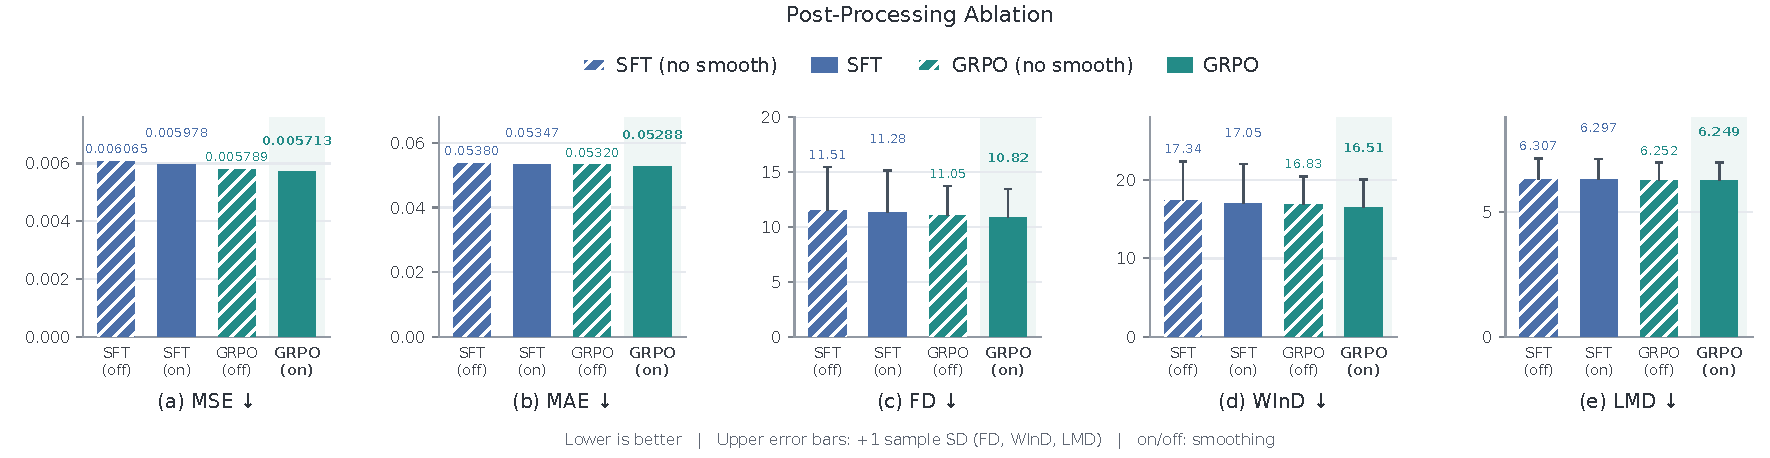
\includegraphics[width=\linewidth]{figures/ablation_smoothing_wide.pdf}
    \caption{The refinement gain is not a smoothing artifact. Turning smoothing off shifts both generators by a small and similar amount, and the refined generator without smoothing still outperforms the supervised generator with it. Lower is better, and hatching identifies the no-smooth variants.}
    \label{fig:ablation_smoothing}
\end{figure}

\subsection{Effect of Inference-Time Post-Processing}
\label{sec:ana_post}

Because AudioMouth generates each unit independently and then concatenates them, a reader may reasonably suspect that its advantage originates in the filtering applied afterwards instead of in what the model learned. To settle this, we evaluate the supervised and refined generators with and without $f_{\mathrm{post}}(\cdot)$, which gives a crossed comparison in which the effect of refinement can be read at both levels of post-processing.

As shown in Figure~\ref{fig:ablation_smoothing}, post-processing produces small improvements for both generators, and the refined generator without any smoothing still outperforms the supervised generator with it on every metric. The two mechanisms therefore do not overlap. Filtering removes high-frequency jitter and the small discontinuities left at unit boundaries, which is a property of the output signal and is available to any method that emits piecewise trajectories. Refinement changes the generator itself through feedback on complete decoded sequences during training, which is why its benefit survives when the filter is switched off. The results show that the refinement gains persist without smoothing, demonstrating the advantage of treating post-processing as a complement to motion-aware learning instead of a substitute for it.

\section{Limitations and Future Work}
\label{app:limitations}

\noindent\textbf{Linguistic Input at Test Time.}\quad
Our BEAT evaluation supplies dataset-provided word and phoneme annotations at test time, so the reported numbers measure the generation stage under correct linguistic input and do not yet establish robustness to recognition errors. The baselines in Table~\ref{tab:main} consume audio alone, so part of the reported margin reflects the additional information available to our model. This is a property of the formulation we are proposing and not an incidental advantage, since the framework is built around linguistic conditioning, but it means the comparison should be read as a comparison of formulations. Quantifying the degradation under automatically recognized transcripts and phonemes is the most important remaining experiment, and the general pipeline of Eq.(\ref{eq:seg}) is already defined for that setting.

\noindent\textbf{Baseline Adaptation.}\quad
Three of the four baselines are evaluated with released weights because their training code or data is unavailable, so they are not adapted to the speakers and capture conditions of our split while our model is. The ablations in Sec.\ref{sec:analysis} are therefore the evidence for our specific design choices, since they hold the backbone, the data, and the objective fixed, while Table~\ref{tab:main} situates the method against methods as they are distributed.

\noindent\textbf{Statistical Resolution.}\quad
The reported differences are means over a few dozen evaluation scripts without significance testing, which is sufficient for the large margins in Table~\ref{tab:main} and in the conditioning and reweighting ablations, and is not sufficient to resolve the few-percent mean differences produced by refinement. Our reading of that stage in Sec.\ref{sec:ana_grpo} therefore rests on the reduction in across-script dispersion, which is a larger effect.

\noindent\textbf{Evaluation Scope.}\quad
All five metrics compare a prediction against one reference trajectory, so none of them measures perceived synchronization or naturalness, and we report no user study and no audio-visual offset metric. Our outputs are also quantized to eleven levels per coefficient, which removes capture noise from the prediction as a side effect, so part of the frame-level margin in Table~\ref{tab:main} may reflect that smoothing instead of better articulation. Both gaps are addressable with a perceptual study and an unquantized variant, and neither is settled by the present results.

\noindent\textbf{Scope and Cost.}\quad
The current scope covers 32 mouth-related ARKit coefficients, a fixed geometry basis for the reward, and a single English corpus. Autoregressive JSON generation produces one token per coefficient value, so output length grows linearly with duration and the inference cost of a 30B backbone has not been characterized for real-time deployment. SLMD remains a surrogate for mouth deformation, and although Sec.\ref{sec:ana_slmd} shows it is necessary for stable refinement, it is not equivalent to the rendered landmark metric.

\noindent\textbf{Future Work.}\quad
We plan to characterize the pipeline under recognized instead of annotated linguistic input, to extend generation to full-face coefficients, to use the instruction-following ability of the backbone for explicit emotional control through natural language, and to reduce inference cost so that the formulation becomes practical for interactive use.


\end{document}
